\chapter{INTRODUCTION}
\doublespacing
\section{Problem Statement}
\hspace{0.5in}Model performance in machine learning is heavily dependent upon the availability of training data. Furthermore, in situ applications of machine learning require data to be indicative of the real world environment the applications plan to infer in. For buried object detection, this would be a B-scan image that bears a close resemblance to B-scans collected in the field. However, these data are not widely available, and when available, the number of samples is few. In situations like this, data augmentation can produce many samples to enhance classification of buried objects  \cite{DBLP}. In the world of Ground Penetrating Radar, an open source software named \textit{gprMax} is used to simulate the presence of underground objects \cite{gprMax}. This software is based on \acrfull{fdtd} \cite{FDTD}, a numerical method to solve Maxwell's equations that govern waves propagation within a specific medium. The problem with this type of simulated data is that it bears little resemblance to a B-scan that would be obtained in the real world. Furthermore, due to the complexity of \acrshort{fdtd}, time to complete a single simulation can take several hours. Thus making the synthesis of a large set of images for training data, virtually impossible. To solve this problem, we propose a novel generative model architecture to synthesize realistic B-scans in real time. In addition, to benchmark the generative model, a classifier is produced that is capable of running in real time on an edge server.

\section{Significance of the Study}
\hspace{0.5in}The significance of this study is to demonstrate that generative models can be successfully applied to GPR data. Furthermore, the generated data can be used in lieu of field collected samples to improve classifiers for the detection of underground objects.

\section{Objectives of the Study}
\hspace{0.5in}The objectives of this study are three fold. The first is to establish a generative architecture for the generation of pseudo realistic B-scans. The second is to develop a real time classifier, capable of being deployed on an edge sever. The final is to incorporate frequency information into time-domain architectures.

\section{Proposed Approach}
\hspace{0.5in}In this thesis, \acrfull{gans} will be investigated for \acrshort{gpr} data augmentation for object identification. Both simulated and real \acrshort{gpr} data will be considered as inputs to the generator of a GAN to generate realistic \acrshort{gpr} data. Based on the feature analysis of \acrshort{gpr} data, a novel objective function and the architecture of GAN are proposed. An algorithm for GAN training with different types of training data is developed. The impact of GAN-synthesized data on the performance of \acrshort{gpr} image classification is evaluated. To the best knowledge of the authors, very few work has been done on studying \acrshort{gans} for \acrshort{gpr} data analysis in a united framework combining data augmentation and data classification. A detailed diagram of the overall system structure is depicted in Figure \ref{fig:GAN_Architecture}
\vspace{0.5\baselineskip}
\begin{figure}[H]
  \centering
  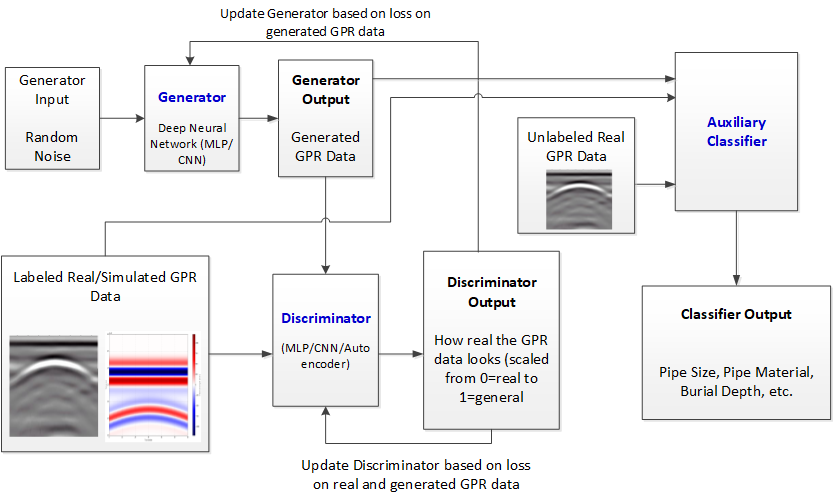
\includegraphics[width=1.0\linewidth]{figures/GAN_Figure.png}
  \caption{\\Proposed GAN Architecture}
  \label{fig:GAN_Architecture}
\end{figure}
\section{Organization of Thesis}
\hspace{0.5in}The remainder of the thesis is organized as follows: Chapter 2 begins with an introduction to theoretical background for the information contained herein. Chapter 3 is the proposed methodology of the experiments is established along with the architectures of the proposed models. Chapter 4 is the discussion of the results. In Chapter 5, the thesis is concluded with final thoughts and an outline for future work.